\documentclass[11pt]{article}

\usepackage[margin=1in]{geometry}
\usepackage{graphicx}
\usepackage{amsmath}
\usepackage{amssymb}
\usepackage{booktabs}
\usepackage{natbib}
\usepackage{hyperref}
\usepackage{setspace}

\graphicspath{{plots/}}
\setstretch{1.1}

\title{Action Chunking as Conditional Policy Compression in Rock--Paper--Scissors}
\author{Daniel Mulford \and Kristen Lee \and Sara Tsai}
\date{\today}

\begin{document}

\maketitle

\begin{abstract}
Chunking is a strategy for grouping units of information in memory and is widely believed to reduce cognitive load under working-memory constraints. Recent work attempts to formalize chunking in terms of Shannon information: an agent's policy can be modeled as a noisy communication channel in which the agent optimizes a tradeoff between fidelity and bitrate \citep{gershman2021reward}. Using a simple stimulus--response task, \citet{lai2025action} demonstrate that human chunking is governed by conditional policy complexity, a quantity they define as the mutual information between state and action after conditioning on one previous timestep of state history. Implicit in their account is the suggestion that, in more complex tasks, chunking may be governed by information extending further back in time. We attempt to provide explicit evidence for this hypothesis. Participants played 100 rounds of Rock--Paper--Scissors against a computer opponent whose hidden policy consisted of chunked sequences of variable length $L \in \{2, 3, 4, 5\}$. Win rate increased with chunk length ($R^2 = 0.585$, $p = 0.027$), while reaction time showed an inverse U-shaped relationship that peaked at $L = 3$ ($R^2 = 0.722$, $p = 0.041$). We argue that these patterns are consistent with the idea that our participants optimized specifically for policy complexity conditioned on a multi-step history.
\end{abstract}

\section{Introduction}

Chunking has long been proposed as a mechanism for coping with the limited capacity of working memory. In Miller's classic formulation, recoding multiple items into a single chunk can increase the amount of usable information without increasing the apparent burden on short-term memory \citep{miller1956magical}. Since then, chunking has been documented across a wide range of domains, from verbal learning to expertise in chess, and has been implemented in computational models such as CHREST \citep{gobet2001chunking}. In sequential action settings, chunking is often associated with faster and more automatic responding because a series of actions can be executed as a unit rather than selected one-by-one \citep{dezfouli2012habits}.

Recent work has reframed these ideas in information-theoretic terms. Building on Miller's work, \citep{mathy2012compression} constructed digit sequences with variable information content using ``runs'' of ascending or descending digits, and observed that total sequence length \emph{after} compression was a better predictor of recall than raw digit span, citing about 3-4 distinct chunks as the limit. From a RL perspective, \citet{gershman2021reward} model action selection as a communication problem in which a policy maps states to actions under a signal bandwidth constraint. In that framework, policy complexity is quantified by the mutual information between states and actions,
\[
I(S;A) = \sum_{s,a} p(s,a)\log \frac{p(a \mid s)}{p(a)},
\]
and capacity limits imply a reward--complexity trade-off. Extending this idea to action chunking, \citet{lai2025action} argue that temporal structure can reduce the coding cost of a policy. Their account focuses on conditional policy complexity, in which the cost of selecting an action is reduced after conditioning on the immediately preceding state.

\begin{figure*}[t]
    \centering
    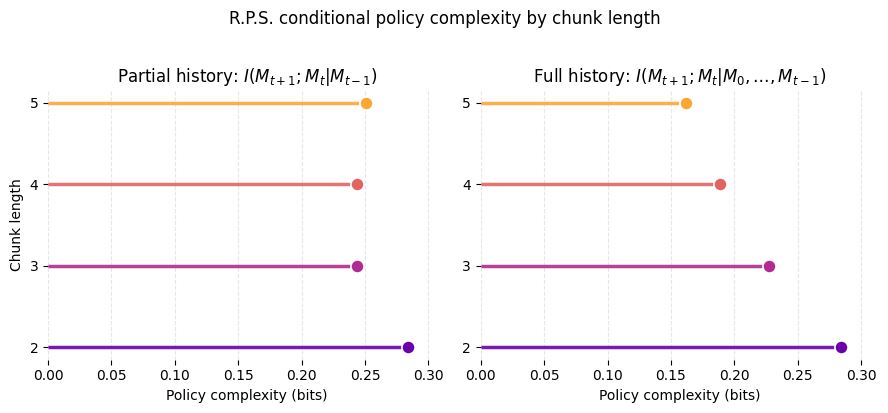
\includegraphics[width=\textwidth]{cpc.png}
    \caption{Comparison of policy-complexity measures across chunk lengths. Full-history conditioning distinguishes each condition of  our task more clearly than a one-step conditional measure.}
    \label{fig:cpc}
\end{figure*}

This framework raises a natural question: what happens when successful prediction depends on more than one previous timestep? The real world constantly asks us to make choices that depend on information that may not be immediately available. If chunking is driven by representational cost, those representations should properly account for all information relevant to the task.

We tested this idea in a Rock--Paper--Scissors (RPS) task with a partially deterministic computer opponent. The opponent played random moves until a hidden key move occurred, after which it emitted a deterministic chunk of length $L$. This design preserved uncertainty while creating stretches of predictable play that could, in principle, be learned and exploited by participants. Because the hidden phase of the policy cannot always be inferred from only the last move, our task distinguishes one-step conditional policy complexity from a fuller history-conditioned quantity (see the discussion for details). We predicted that conditions with greater chunk length would yield higher accuracy and shorter reaction times.

\section{Methods}

\subsection{Task}

Participants completed 100 rounds of RPS against a browser-based computer opponent. The opponent's hidden policy was defined by a chunk length $L$ and a key move $K$. While not in a chunk, the opponent sampled uniformly at random from \{\emph{rock}, \emph{paper}, \emph{scissors}\}. If the sampled move was not $K$, play remained random on the next trial. If the sampled move was $K$, the opponent entered a deterministic chunk of length $L$: the key move was followed by a fixed sequence of $L-1$ additional moves, after which the policy returned to random play.

To distinguish random from predictable periods, we assigned each trial a \emph{policy phase} $\phi$. Trials generated during random play were labeled $\phi = 0$. Trials that followed the key move within a deterministic chunk were labeled $\phi \in \{1,\ldots,L-1\}$. The latter trials were the rounds on which an attentive participant could, in principle, anticipate the computer's next move.

Participants were presented with instructions at the beginning of the experiment and were explicitly told that the purpose of this Rock, Paper, Scissors task game was to learn how people learn and utilize chunking structure in a computer game. Instructions included that players must respond before the end of a 3 second countdown, using keys \texttt{R}, \texttt{P}, and \texttt{S} to represent the moves `Rock', `Paper', and `Scissors', respectively. After the countdown concludes, or the player inputs a response, the computer displays its move and the result of the match (`Win', `Tie', `Loss') for 1500 ms. The instructions also informed participants that the computer did not play randomly, with key moves triggering a consistent pattern. Players were then presented with a practice trial with a provided example chunk structure ($[\text{Rock}, \text{Paper}, \text{Paper}]$) to familiarize themselves with the task flow. After successfully identifying this practice sequence twice, players could begin the scored trials. 


\subsection{Measures and exclusions}

Our primary dependent variables were reaction time and accuracy. Accuracy was defined as the participant's average win rate on deterministic rounds only, that is, trials with $\phi > 0$. This effectively normalized accuracy to a maximum of 100\%.

The analysis assumed that retained responses reflected successful policy learning. We therefore kept only responses with at least 70\% accuracy on deterministic rounds in the second half of the task. After learning that one participant had inspected the JavaScript console during the experiment, we conservatively excluded all responses with greater than 95\% overall accuracy. These filters were intended to remove both non-learners and likely invalid near-perfect runs.

\subsection{Design and sample}

The original design was between-subjects: each participant was to be assigned a single chunk-length condition with $L \in \{2,3,4,5\}$. In practice, recruitment constraints made that design difficult to sustain, so participants were permitted to submit multiple responses. The unit of analysis in this draft is therefore the response rather than the participant.

We recruited a convenience sample of volunteers and obtained 48 total responses. After applying the learning and validity filters described above, 8 responses remained for analysis. See section~\ref{sec:discussion} for more details on the challenges related to sample size.

\subsection{Policy-complexity analysis}

The theoretical motivation for the experiment was that the computer opponent's move process varies in informational complexity across chunk lengths. At the coarsest level, the dependence between consecutive opponent moves can be described by
\[
I(M_t; M_{t+1}),
\]
where $M_t \in \{\text{rock}, \text{paper}, \text{scissors}\}$ is the opponent's move at time $t$. However, predicting the next move requires more than the current move alone. In particular, the key move marks the start of a deterministic run, so the player must condition their expectation on a state history at least as far back as the key move during the chunking phase.

To evaluate this claim, we computed conditional policy complexity for the hidden opponent process in two ways. First, we considered a one-step quantity, $I(M_t; M_{t+1} \mid M_{t-1})$, which parallels the formulation emphasized by \citet{lai2025action}. Second, we considered a full-history quantity, $I(M_t; M_{t+1} \mid M_0, \ldots, M_{t-1})$, which conditions on all preceding moves in the current sequence. These quantities were calculated exactly by exhaustive enumeration of all hidden policies for each chunk length and independently checked using a simulation of 30{,}000 rounds across 256 sampled policies per condition. Source code for the experiment and analyses is available at \url{https://github.com/kristen-lee-120/rps}.

\section{Results}

Figure~\ref{fig:behavior} shows the relationship between chunk length and both behavioral outcomes. In the left panel, accuracy on deterministic rounds increased with chunk length ($R^2 = 0.585$, $p = 0.027$). Participants therefore appeared to perform better when the hidden policy contained longer deterministic stretches.

Reaction time showed a more nuanced pattern (Figure~\ref{fig:behavior}, right panel). Instead of decreasing monotonically with chunk length, reaction time followed an inverse U-shaped trend that peaked at $L=3$ ($R^2 = 0.722$, $p = 0.041$). Even so, the overall shape is consistent with the idea that chunk length modulates the computational demands of the task, albeit not in a perfectly linear way.

\begin{figure*}[t]
    \centering
    \begin{minipage}[t]{0.495\textwidth}
        \centering
        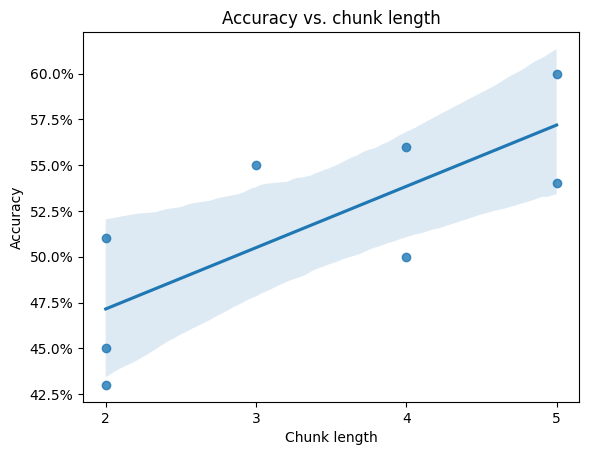
\includegraphics[width=\linewidth]{acc_vs_L.png}
    \end{minipage}\hfill
    \begin{minipage}[t]{0.495\textwidth}
        \centering
        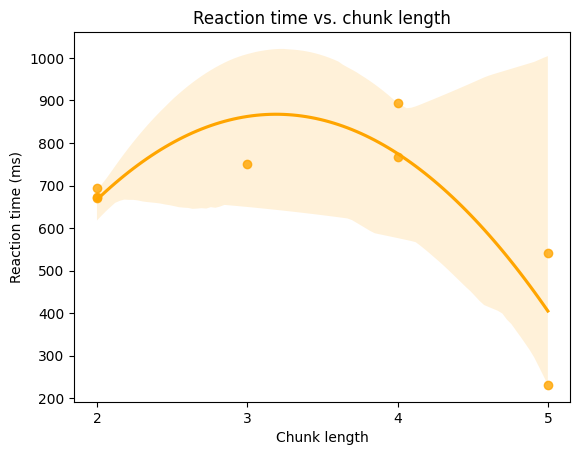
\includegraphics[width=\linewidth]{rt_vs_L.png}
    \end{minipage}
    \caption{Behavioral results as a function of chunk length. Left: accuracy on deterministic rounds increased with chunk length, with a positive fitted trend ($R^2 = 0.585$, $p = 0.027$). Right: mean reaction time followed an inverse U-shaped relationship, with the peak centered around $L=3$ ($R^2 = 0.722$, $p = 0.041$).}
    \label{fig:behavior}
\end{figure*}

Because only 8 responses survived filtering, these results should be interpreted as preliminary. The positive accuracy trend is the clearest behavioral signal in the dataset. The reaction-time effect is suggestive but less cleanly aligned with a simple monotonic complexity account, particularly at shorter chunk lengths where the ease of learning the short hidden sequence may have overshadowed the policy compression effects.

\section{Discussion}

\label{sec:discussion}

\subsection{Implications for conditional policy complexity}

Our results both reinforce the interpretation of chunking as conditional policy compression developed in \citet{gershman2021reward} and \citet{lai2025action}, and provide evidence for a slightly more general formulation of policy complexity.

The player facing our RPS opponent does not merely need to know its most recent move; they need to know whether and when the key move has occurred. Consistently tracking that latent phase requires conditioning on at least $L$ previous moves.

This distinction is illustrated in Figure~\ref{fig:cpc}. Exact calculations over the hidden-policy space showed that the full-history conditional quantity decreased monotonically with chunk length, from approximately 0.284 bits at $L=2$ to 0.162 bits at $L=5$. By contrast, the one-step conditional quantity remained clustered in a narrower range (roughly 0.24--0.28 bits) and did not cleanly separate all four chunk-length conditions. In other words, multi-step conditional policy complexity formalizes the cognitive requirements of our RPS task.

The results therefore suggest a practical relationship between chunking and this broader notion of policy complexity. Accuracy improved as chunk length increased, matching the decrease in full-history conditional information. Reaction time did not decrease monotonically, but the deviation is not fatal to the account. Short chunks may be easy to learn quickly, producing relatively fast responses despite weaker compression benefits, while intermediate chunks may temporarily impose the greatest monitoring cost before longer deterministic sequences become more exploitable. With a larger sample and a refined task design, it would be possible to test this explanation more directly.

\subsection{Limitations}

Our most significant challenge was gathering sufficient data. Only 8 of 48 responses remained after filtering. This small sample size may result in low power, even though our effects are statistically significant according to the usual $p<0.05$ criterion.

Ultimately, we had to balance the competing interests of keeping participants engaged with the task and implementing enough trials to gather sufficient data, leading us to a between-subjects design with 100 scored trials per session. This introduced the usual concerns with a between-subjects design including higher variance and fewer total data points per condition, and may have provided insufficient time for participants to master their randomly assigned hidden sequence. However, we were concerned about participants fatiguing or disengaging if tasked with more trials.

Additionally, as we monitored the feedback provided by participants during the data collection phase, several points of confusion surfaced. Some people didn't realize that the pattern differed from the practice trial or thought that the chunk pattern changed throughout the experiment. Furthermore, early feedback indicated that our initial interface which failed to distinguish ties from losses was confusing. Accordingly, we updated the instruction screens after we had collected approximately 25 of our eventual 48 total responses to address these problems. This means the final dataset may mix better-understood later responses with noisier earlier ones.

In order to compensate for challenges gathering enough high-quality responses, as mentioned in the methods section, we allowed participants to submit multiple responses. Several of the participants that performed the experiment in-person were also given additional coaching and therefore had an advantage over anonymous online participants in terms of task understanding. We reasoned that these responses would not confound our results because they would be evenly distributed across all conditions randomly, and our data cleaning process explicitly filtered out all participants with poor task understanding regardless.

\subsection{Future design considerations}

Because understanding the scheme of our RPS game and learning the hidden pattern was a significant bottleneck in collecting useable data, future iterations of the experiment should generally make the objective of the task more transparent. In addition to providing more practice trials and more thorough instructions, we speculate that a more intuitive way of specifying \emph{rock}, \emph{paper}, or \emph{scissors} may be helpful. For example, a touchscreen with visual icons may be easier than learning the keys \texttt{R}, \texttt{P}, or \texttt{S}.

Providing greater incentives for participation, such as further gamifying the experiment with a points-based system, may enable study designs that require more time and attention from each participant. In particular, a within-subjects design in which each participant completes all four conditions in random order would allow for much more precise effect estimates.

\section{Conclusion}

This study provides preliminary evidence that chunking in a sequential RPS task is associated with multi-step conditional policy compression. Accuracy improved with chunk length, and reaction time varied systematically across chunk conditions, while exact complexity calculations showed that only a full-history conditional measure clearly distinguished the hidden policies used in the experiment. Given the small number of retained responses, these findings should be treated as suggestive rather than definitive. Even so, they provide additional support for the formulation of chunking as policy compression generally, and evidence that policy complexity is conditioned on all relevant state history.

\newpage 
\bibliographystyle{plainnat}
\bibliography{references}

\end{document}
